\documentclass[preprint,12pt,times,nonatbib]{elsarticle}
\usepackage[T1]{fontenc}
\usepackage[utf8]{inputenc}
\usepackage{amsmath,amssymb,amsthm,booktabs,array,graphicx,microtype,xcolor}
\usepackage[style=numeric-comp,sorting=none,backend=biber,sortcites=true,giveninits=true,maxbibnames=99]{biblatex}
\addbibresource{references.bib}
\usepackage{xurl}
\usepackage[hidelinks]{hyperref}
\usepackage{placeins,geometry,needspace}
\makeatletter
\newcommand{\captionof}[1]{\def\@captype{#1}\caption}
\setlength{\@fptop}{0pt}
\setlength{\@dblfptop}{0pt}
\makeatother
\renewcommand{\topfraction}{0.9}
\renewcommand{\dbltopfraction}{0.9}
\renewcommand{\textfraction}{0.08}
\renewcommand{\floatpagefraction}{0.8}
\renewcommand{\dblfloatpagefraction}{0.8}
\setlength{\dbltextfloatsep}{14pt plus 2pt minus 2pt}
\setlength{\textfloatsep}{14pt plus 2pt minus 2pt}
\raggedbottom
\geometry{a4paper,left=23mm,right=23mm,top=23mm,bottom=23mm}
\journal{Neurocomputing}
\newtheorem{proposition}{Proposition}
\newtheorem{lemma}{Lemma}
\newcommand{\R}{\mathbb R}
\newcommand{\rms}{\operatorname{rms}}
\newcommand{\QUART}{\mathrm{QUART}}
\setlength{\emergencystretch}{1.5em}
\setlength{\tabcolsep}{4pt}
\usepackage{needspace}
\begin{document}
\begin{frontmatter}
\title{QUART: Exact control of forecast revisions in online learning}
\author[a]{Yanbo Bian\corref{cor1}}
\ead{24722081@bjtu.edu.cn}
\author[b]{Zhihai Wang}
\ead{zhhwang@bjtu.edu.cn}
\cortext[cor1]{Corresponding author.}
\address[a]{Computer Science and Technology, Weihai International Academy, Beijing Jiaotong University, 69 Xiandai Road, Nanhai New Area, Weihai, Shandong 264401, China.}
\address[b]{School of Computer Science and Technology, Beijing Jiaotong University, 3 Shangyuancun, Haidian District, Beijing 100044, China.}
\begin{abstract}
Online forecasters learn from past errors while changing predictions whose outcomes remain unknown. Here we introduce QUART (query-aware updates with adaptive revision truncation), which bounds each update at the current, unlabelled forecast query. QUART takes the largest feasible fraction of a normalised residual-learning proposal under an explicit displacement budget. Its effective-operator recurrence preserves observed-feedback loss non-increase and removes redundant gated factorisations while the source forecaster remains frozen. Across three electricity-demand datasets, two frozen forecasters and five seeds, all 23,375 active updates met the budget within numerical tolerance. Matched-step historical clipping exceeded the same budget in 13.00\% of benchmark updates and 24.29\% of entity-transfer updates. Across 12 benchmark settings, mean relative differences in mean absolute error (MAE) were $-4.02\%$ against frozen forecasting and $-0.74\%$ against independently tuned normalised least mean squares (NLMS; 95\% CI, $-0.97$ to $-0.53\%$). Across eight new-entity settings, the corresponding differences were $-15.13\%$ against frozen forecasting and $+2.04\%$ against fixed NLMS (95\% CI, $+0.13$ to $+4.36\%$). Five budgets map the accuracy--displacement response. Temporal comparisons remain exploratory; entity-transfer configurations were fixed before scoring. QUART makes forecast revision an explicit design variable in online learning.
\end{abstract}
\begin{keyword}
Electricity-demand forecasting \sep Online calibration \sep Test-time adaptation \sep Delayed feedback \sep Adaptive filtering \sep Forecast stability
\end{keyword}
\end{frontmatter}


\section{Introduction}
Online forecasting learns from completed outcomes while revising predictions whose targets remain unknown. Electricity-demand systems issue daily and weekly forecasts before earlier outcomes are fully available \parencite{baydan2026operational,antoniadis2024hierarchical}. Once an earlier horizon completes, its error updates a forecast for a different trajectory.

Forecast architectures and distribution-aware normalisation capture temporal structure and accommodate changing distributions \parencite{zeng2023transformers,nie2023patchtst,liu2022nonstationary,fan2023dishts,chen2024calibration}. Test-time adaptation updates input or output corrections as labels arrive \parencite{kim2025tta,im2026cosa}. Yet reducing a historical residual does not determine how far the current forecast moves. Equivalent initial predictors can also respond differently to the same parameter step \parencite{amari1998}. The current forecast provides a direct point of control for this change.

We introduce QUART (Query-aware Updates with Adaptive Revision Truncation), an online residual calibrator that limits each learning step at the current, unlabelled query. It specialises prediction-space update control \parencite{schulman2015trpo} for deterministic forecasting with delayed feedback. A normalised adaptive-filtering proposal defines the learning direction \parencite{nagumo1967}, and its effect on the current query sets the largest admissible fraction. The closed-form recurrence enforces a displacement budget while preserving observed-feedback loss non-increase. An effective calibration operator removes dependence on redundant gated factorisations without updating the frozen source forecaster.

Across regional, customer and household demand, we measure forecast displacement, prediction error and calibration cost. Expanded comparator searches and matched update rules isolate current-query control; five budgets map the accuracy--displacement response. Transfer to new entities tests whether the bound persists when the predictive response changes.

\section{Related work}
\subsection{Forecast structure and distribution change}
Forecast structure is represented through decomposition, patches, temporal variation and variable-wise attention \parencite{zeng2023transformers,nie2023patchtst,wu2023timesnet,liu2023itransformer}. Adaptive decomposition, multiresolution mixing and clustering further extend these representations \parencite{hu2025adaptive,murad2025wpmixer,qiu2025duet}. This architectural diversity motivates calibration interfaces that act on fixed predictions while leaving the source architecture intact.

Distribution-aware methods recover information affected by normalisation and temporal shift \parencite{liu2022nonstationary,fan2023dishts,chen2024calibration,he2025robust}. Affine prototypes and shift-aware optimisation extend this approach \parencite{apt2026,adamshift2026}. These methods address changing data distributions, whereas QUART bounds the displacement caused by each calibration update at the current query.

\subsection{Forecast adaptation with delayed outcomes}
Continual test-time adaptation examines how updates accumulate during deployment \parencite{wang2022continualtta}. For forecasting, TAFAS combines period-aware scheduling with input and output calibration \parencite{kim2025tta}. COSA provides a context-aware output map \parencite{im2026cosa}, whereas AdaNODEs uses a dynamical formulation \parencite{adanodes2026}. PADRE guides updates with delayed residual evidence \parencite{li2026padre}, and frequency-aware calibration emphasises the timing of matured supervision \parencite{wang2026fac}.

These methods calibrate trained forecasters for evolving streams of data. We compare output updates under identical frozen predictions, available context and matured feedback. COSA uses its released linear module under this shared schedule, excluding native scheduling and retrospective forecast replacement.

\subsection{Adaptive filtering and update constraints}
Normalised adaptive filtering scales updates by the energy of the training input \parencite{nagumo1967}. Set-membership normalised LMS selects updates under feedback-error constraints, including time-varying error bounds \parencite{gollamudi1998setmembership,delamare2009setmembership}. Parameter-space trust regions constrain optimisation steps through a chosen parameter metric \parencite{more1983trustregion}. Spectral constraints and compact parameterisations provide further choices of representation \parencite{miyato2018spectral,hu2021lora,ding2023peft}. Trust region policy optimisation constrains represented outputs by bounding KL divergence between stochastic policies \parencite{schulman2015trpo}.

QUART applies prediction-space control to delayed-feedback forecasting through an affine effective operator. This operator gives the exact current-query displacement of an NLMS proposal, yielding the largest feasible fraction in closed form. The protected forecast is unlabelled, whereas the historical input supplies the learning signal. Matched-step NLMS and matched-step historical clipping distinguish current-query control from unconstrained and feedback-based scaling. Historical clipping serves as a diagnostic control for this distinction.

\section{Query-aware updates with adaptive revision truncation}
\subsection{Delayed feedback and the calibration operator}
At origin $t$, a frozen forecaster uses the preceding $L=336$ hours of loads and calendar covariates to predict $p_t\in\R^{H\times d}$. Forecast horizons are $H\in\{24,168\}$, and observed training statistics standardise the loads. For channel $j$, the source trajectory $p_{t,j}\in\R^H$ defines the feature vector
\begin{equation}
 q_{t,j}=[p_{t,j}^{\mathsf T},c_t^{\mathsf T},1]^{\mathsf T}\in\R^{H+6},
\end{equation}
where $c_t\in\R^5$ summarises loads observed before the forecast origin. Its entries average the $H$ hours preceding indices $t,t-24,\ldots,t-96$, pooling observed standardised values across channels.

Each channel has an effective operator $C_{t,j}\in\R^{H\times(H+6)}$, initialised to zero. The operator produces the calibrated forecast
\begin{equation}\label{eq:forecast}
 \widehat y_{t,j}=p_{t,j}+C_{t,j}q_{t,j}.
\end{equation}
Forecasts are issued every 24 h. Feedback from origin $s$ becomes eligible once $s+H\leq t$, using the stored source prediction and context to define $z_j=q_{s,j}$. The outcome $y_{s,j}$ and observation mask $m_{s,j}$ determine the available feedback. Each eligible forecast is consumed once, while previously issued predictions remain fixed (Fig.~\ref{fig:method}).


\begin{figure}[!htbp]
\centering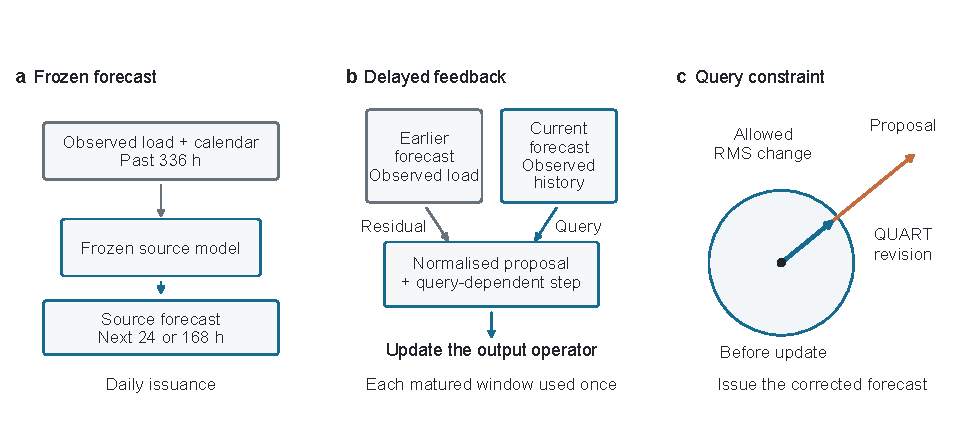
\includegraphics[width=\textwidth]{figures/fig1_method.pdf}
\caption{\textbf{Delayed feedback sets the learning direction; the current query sets the limit.} (a) A frozen source predicts the next 24 or 168 h from 336 h of observed history. (b) A completed forecast supplies feedback, and the current source forecast supplies the query. (c) QUART scales a normalised proposal to bound the resulting change in the current forecast. Forecasts are issued daily with delayed feedback. Schematic code was prepared with OpenAI Codex (CLI 0.162.0-alpha.2).}
\label{fig:method}
\end{figure}


\subsection{Forecast-equivalent initialisation and update sensitivity}
A gated adapter predicts $p+\tanh(g)(Wq+b)$. At $g=0$, all residual maps produce the same initial forecast. Scaling $W,b$ therefore changes the representation while leaving that prediction unchanged.

\begin{lemma}[Initial gated-step sensitivity]\label{lem:gate}
For one channel, let $f=p+\tanh(g)v$, where $v=Wz+b$ and $r=y-p$, and use loss $\frac12\|f-y\|_2^2$. Starting at $g=0$, one unregularised gradient step of size $\eta$ changes the forecast on that same input by
\begin{equation}
 \eta vv^{\mathsf T}r+O(\eta^3).
\end{equation}
Replacing $(W,b)$ with $(aW,ab)$ leaves the initial forecast unchanged and multiplies the leading update term by $a^2$.
\end{lemma}

The lemma establishes representation sensitivity for a gradient step, whereas the experiments test the released Adam-based implementation. Both distinguish equivalent initial forecasts from subsequent update behaviour. The intervention uses $a\in\{0.1,1,10\}$ with identical data, initial forecasts and selected optimisation settings.

\subsection{Normalised learning with current-query control}
At a feedback event, the masked residual under the current operator is
\begin{equation}
 r_j=m_{s,j}\odot(y_{s,j}-p_{s,j}-C_{t,j}z_j).
\end{equation}
For $0<\eta\leq1$, define the normalised proposal
\begin{equation}\label{eq:direction}
 D_j=\eta\frac{r_jz_j^{\mathsf T}}{1+\|z_j\|_2^2}.
\end{equation}
Without $\eta$, the proposal minimises a ridge-regularised correction objective for one feedback sample. This normalised least-mean-squares direction leaves unobserved target rows unchanged.

The proposal acts on the current forecast through
\begin{equation}\label{eq:transfer}
 v_j=D_jq_{t,j}
 =\eta r_j\frac{z_j^{\mathsf T}q_{t,j}}{1+\|z_j\|_2^2}.
\end{equation}
The proposed change depends on both the feedback magnitude and the alignment of the historical feature with the current query. Historical-feature normalisation alone does not enforce the prescribed displacement budget at another query. Stack the vectors as $V\in\R^{H\times d}$ and define $\rms(V)=\|V\|_F/\sqrt{Hd}$. The displacement budget is
\begin{equation}
 B_t=\rho\max\{1,\rms(p_t)\},\qquad \rho=0.05.
\end{equation}
QUART takes the largest admissible fraction of the proposal along this direction:
\begin{equation}\label{eq:query}
 \beta_t=\min\left\{1,\frac{B_t}{\rms(V)}\right\},\quad
 C_{t,j}^{+}=C_{t,j}+\beta_tD_j,
\end{equation}
with $\beta_t=1$ when $V=0$. The updated operator $C_t^{+}$ then produces the forecast at the same current query. Equation~\eqref{eq:query} selects a scalar step along the normalised proposal ray from the source prediction and matured feedback, without requiring future targets.

\Needspace{12\baselineskip}
\begin{proposition}[Descent, current-query control and factorisation invariance]\label{prop:control}
For fixed available features and an observed feedback mask, the QUART step satisfies:
\begin{enumerate}
\item the squared error on every observed feedback channel is non-increasing;
\item $\rms(\widehat y_t^{+}-\widehat y_t)\leq B_t$;
\item two factorisations encoding the same initial operators $C_{0,j}$ generate identical operator and forecast trajectories under the same observations, masks, queries and step sizes.
\end{enumerate}
\end{proposition}

The proof follows from $r_j^{+}=(1-\kappa_j)r_j$ on observed entries, where
\begin{equation}
 \kappa_j=\beta_t\eta\frac{\|z_j\|_2^2}{1+\|z_j\|_2^2}\in[0,1],
\end{equation}
and the definition of $\beta_t$. The effective map $C$ determines the recurrence; Supplementary Section S1 provides the full derivation. The bound applies to joint-channel, standardised displacement across one feedback update at a fixed origin and query. Physical-unit channel limits and changes between issuance times require separate specifications.

\subsection{Implementation and matched controls}
QUART stores $dH(H+6)$ coefficients and uses matrix--vector products and rank-one updates without source-model backpropagation. The primary budget is $\rho=0.05$. QUART and independently tuned NLMS select step sizes from $\{0.005,0.02,0.05,0.2,0.4,0.8,1\}$, with a no-update option. NLMS uses the same proposal with $\beta_t=1$.

The historical-feedback clipping control retains the same proposal $D$ but sets
\begin{equation}\label{eq:historical}
 \beta_t^{\mathrm{hist}}=\min\left\{1,
 \frac{\rho\max\{1,\rms(p_s)\}}{\rms([D_jz_j]_{j=1}^d)}\right\}.
\end{equation}
Historical clipping scales the update from the stored forecast and feature, without consulting the current query. Its step size is selected independently from the same seven candidates. Matched controls retain QUART's selected $\eta$ and vary only the admissible fraction, using no constraint or Eq.~\eqref{eq:historical}. These comparisons isolate current-query dependence from general adaptive step scaling. Budget analyses retain every $\rho\in\{0.01,0.025,0.05,0.1,0.2\}$ at the primary step size and after validation selection within each budget.

At each daily origin, QUART computes the source forecast, consumes newly matured feedback and issues the calibrated trajectory once. Stored source predictions and past-context features form the feedback queue; previously issued forecasts remain fixed. At most one feedback window matures per origin on this grid. For 16 channels, float32 operators occupy approximately 0.044 MiB at 24 h and 1.78 MiB at 168 h. These figures exclude the source model and feedback queue. Supplementary Section S1.3 provides the implementation recipe.

\section{Experimental design}
\subsection{Data and frozen source forecasters}
The study spans regional, customer and household demand from EIA-930, ECL and Ausgrid \parencite{eia9302026,uci2015ecl,ratnam2015ausgrid}. Source-order selection retains seven balancing authorities, the first 16 ECL customers and the first 16 Ausgrid general-consumption households. Quarter-hour ECL power is averaged into hourly kW; half-hour Ausgrid energy is summed into hourly intervals. EIA Demand is used directly in MW. Complete hourly axes are retained, with missing inputs filled only from past values. Training means, standard deviations and seasonal MASE scales use observed training entries.

\begin{table}[!tbp]
\centering\small
\caption{Demand scales and evaluation periods. All methods use hourly data, daily forecast origins and identical observed-target masks. Supplementary Section S2 specifies exact hourly boundaries and target coverage for each horizon.}
\label{tab:datasets}
\begin{tabular}{llrl}
\toprule
Dataset & Demand level & Entities & Main scored period\\
\midrule
EIA-930 & Regional (MW) & 7 & January--June 2026\\
ECL & Customer (kW) & 16 & March--December 2014\\
Ausgrid & Household (kWh) & 16 & November 2012--June 2013\\
\midrule
EIA re-evaluation & Regional (MW) & 7 & July--August 2026\\
ECL unused entities & Customer (kW) & 16 & March--December 2014\\
Ausgrid unused entities & Household (kWh) & 16 & November 2012--June 2013\\
\bottomrule
\end{tabular}
\end{table}

EIA source fitting uses 2023--2024, source selection uses 2025 and the original test covers January--June 2026. ECL and Ausgrid use chronological 70\%/10\%/20\% splits. Calibration configurations minimise MAE on the second half of each validation interval. Original benchmark and EIA extension outcomes informed development, making their expanded-grid comparisons exploratory. Supplementary Sections S2--S4 detail this chronology and distinguish the earlier configuration-locked extension.

DLinear and StableShift provide contrasting frozen source representations. DLinear shares trend and seasonal temporal maps across channels \parencite{zeng2023transformers}. StableShift adds linear and neural corrections to a learned daily/seven-day seasonal mixture. It has four temporal-convolution levels, width 128, dilations 1/2/4/8 and a trained rank-eight branch. All source parameters remain frozen, including this branch. Training used AdamW, two learning rates, at most 30 epochs and validation-based early stopping. Supplementary Section S3 and the code archive specify the architectures, settings and checkpoints.

Entity transfer uses ECL MT\_101--MT\_116 and Ausgrid general-consumption customers 101--116, declared before preparation and scoring. These entities are excluded from source fitting and calibration selection. The 60 selected configurations are reused without retraining or retuning, using ascending-ID positional mapping and cohort training-only normalisation. Evaluation uses the same historical calendar as the original cohorts.

\subsection{Controlled comparisons and configuration selection}
COSA uses its released variable-wise linear output module with five historical context values and Adam \parencite{im2026cosa}. We retain its within-event learning-rate rule, dynamic gradient clipping and $10^{-4}$ parameter penalty. Validation crosses starting rates $0.0003/0.001/0.003/0.005$ with 1/5/10/20 update steps. A boundary optimum triggers a validation-only extension to 50 steps or starting rate 0.01, with at most two additional candidates. Every method includes a no-update option. Observed-entry MAE selects configurations separately for each dataset, horizon, source and seed. Supplementary Section S4 reports the complete search and selected configurations.

All methods issue forecasts every 24 h and learn only from fully elapsed earlier horizons, using observed entries when targets are partially missing. COSA's published output module follows this shared schedule without period-dependent scheduling or retrospective replacement. The initialisation intervention scales its residual weights and biases by 0.1, 1 or 10, retaining the zero gate and other settings.

Five seeds, 11/22/33/44/55, yield 60 original source configurations across 12 dataset, horizon and architecture settings. EIA re-evaluation adds 20 configurations and 1,488 hourly observations per region, with 99.67\% observed entries. Entity transfer adds 40 configurations across eight settings. Calibration states reset to zero at the start of each evaluation period.

\subsection{Outcomes and paired inference}
MAE and MSE divide absolute or squared error sums by observed forecast-target counts; RMSE is the square root of MSE. All methods use identical target masks. MASE uses the training-only 24 h seasonal scale. Ten new ECL channels have constant-zero training values. Under unit-standard-deviation normalisation, these channels remain in forecasts, updates, MAE and RMSE. Secondary MASE uses the six channels with defined seasonal scales. Complete-future-block scoring provides a sensitivity analysis.

Paired inference uses 5,000 crossed seed and circular calendar-block draws, with seven-day blocks and 14- and 28-day sensitivities. Shared draws preserve within-dataset dependence across sources and horizons. Each draw recomputes error-sum/count ratios, and macro effects weight settings equally. We report pointwise percentile 95\% intervals and Holm-adjusted tests within separate, predefined comparison families. The intervals describe uncertainty for the evaluated cohorts, fixed source models and recorded adaptation trajectories. Supplementary Sections S4--S7 provide the full inferential definitions and results.

\subsection{Measuring forecast displacement}
For each active update, we measure current-query RMS displacement relative to QUART's budget $B_t$ at the same event. Matching uses dataset, horizon, source, seed and feedback-update index. Matched-step NLMS and matched-step historical clipping share this reference budget. Displacement must exceed $B_t+2\times10^{-6}\max(1,B_t)$ to count as an exceedance, allowing for floating-point tolerance. These post-hoc descriptive summaries include all active events and use empirical quantiles.

\subsection{Analysis and figure preparation}\label{sec:analysis_workflow}
OpenAI Codex (OpenAI, CLI 0.162.0-alpha.2) assisted with analysis and plotting code. Archived Matplotlib scripts generate the plots directly from recorded Source Data and render the method schematic programmatically.

\section{Results}
\subsection{Query control bounds forecast updates}
QUART bounded all 23,375 active updates across the three evaluation phases and preserved observed-feedback loss non-increase within the recorded numerical tolerances. Matched-step historical clipping exceeded the same event budget in 13.00\% of original-benchmark updates and 24.29\% of entity-transfer updates. Matched-step NLMS exceeded it in 43.34\% and 68.05\%, respectively (Table~\ref{tab:control_boundary}). Limiting changes at the historical feedback input therefore permitted larger changes in the current forecast.

\begin{table}[!htbp]
\centering\small
\caption{Current-forecast displacement across evaluation cohorts.}
\label{tab:control_boundary}\begin{tabular}{llrrrr}
\toprule
Evaluation & Update rule & Events & Over budget (\%) & P99 ratio & Max ratio\\
\midrule
Original benchmark & QUART & 12,580 & 0.00 & 1.00 & 1.00\\
 & Matched NLMS & 12,580 & 43.34 & 26.86 & 47.01\\
 & Matched history & 12,580 & 13.00 & 1.50 & 4.31\\
\addlinespace[3pt]
EIA re-evaluation & QUART & 855 & 0.00 & 0.99 & 1.00\\
 & Matched NLMS & 855 & 1.05 & 1.00 & 1.64\\
 & Matched history & 855 & 0.58 & 0.92 & 1.21\\
\addlinespace[3pt]
Unused entities & QUART & 9,940 & 0.00 & 1.00 & 1.00\\
 & Matched NLMS & 9,940 & 68.05 & 78.46 & 146.85\\
 & Matched history & 9,940 & 24.29 & 1.49 & 2.45\\
\bottomrule
\end{tabular}

\par\vspace{3pt}\begin{minipage}{\linewidth}\footnotesize
Each rule is evaluated against QUART's budget at the same origin. Ratios divide RMS displacement by this shared budget. Exceedances allow $2\times10^{-6}\max(1,B_t)$ numerical tolerance. Events include all active matched-step updates; disabled policies contribute none.
\end{minipage}
\end{table}

Historical clipping retained similar prediction error while allowing larger forecast changes. On the original benchmark, its matched-step displacement reached 1.50 times the budget at the 99th percentile and 4.31 at the maximum (Fig.~\ref{fig:mechanism}a). At matched steps, QUART's mean relative MAE difference was $-5.01\%$ against unconstrained NLMS (95\% CI, $-6.28$ to $-3.65\%$). The difference against historical clipping was $-0.11\%$ (95\% CI, $-0.22$ to $-0.02\%$; Fig.~\ref{fig:mechanism}c,d).

Closed-form calibration reduced computational cost relative to controlled COSA. Across 11 active seed-11 settings, the median controlled-COSA-to-QUART calibration-and-scoring time ratio was 19.6 (Fig.~\ref{fig:mechanism}b). Timing used three synchronised unbatched repetitions at the selected update budgets and excluded shared source inference.

\begin{figure}[!htbp]
\centering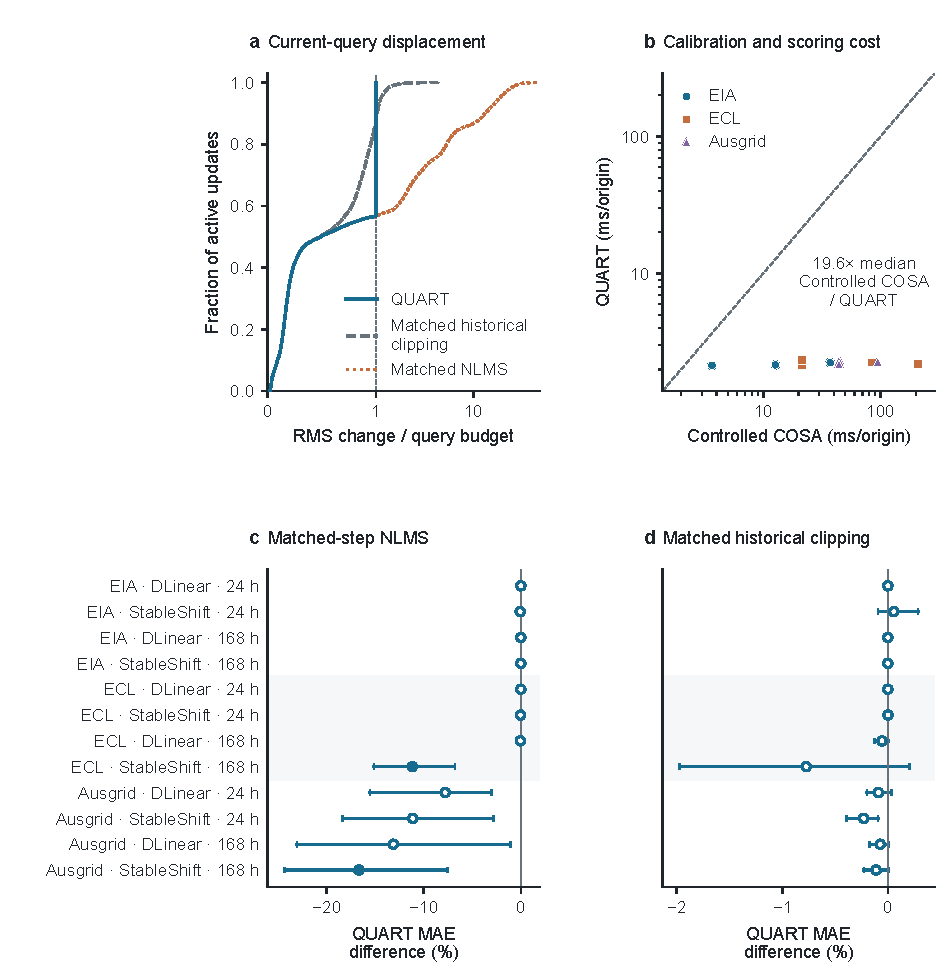
\includegraphics[width=.98\textwidth]{figures/fig2_control_first.pdf}
\caption{\textbf{Forecast displacement, prediction error and calibration cost.} (a) Empirical displacement distributions for QUART, matched-step NLMS and matched-step historical clipping across all active original-benchmark updates. Displacements are normalised by the shared event budget; the reference marks the bound, and comparator tails are retained. (b) Median calibration-and-scoring time over three synchronised unbatched repetitions after warm-up. All 11 seed-11 settings with active QUART and controlled COSA are shown; source inference is excluded. (c,d) Relative MAE differences from matched-step NLMS and matched-step historical clipping across all 12 settings. Bars show pointwise paired 95\% seed/calendar-block intervals. Filled markers meet Holm-adjusted $p<0.05$ in the 48-test matched-control family. Plotting code was prepared with OpenAI Codex (CLI 0.162.0-alpha.2).}
\label{fig:mechanism}
\end{figure}

\FloatBarrier
\subsection{Budget size shapes the accuracy--displacement response}
The five budgets produced a tunable accuracy--displacement response (Fig.~\ref{fig:budget}). At the primary step size, mean relative MAE differences from frozen forecasting were $-3.85\%$ at $\rho=0.01$ and $-2.40\%$ at $\rho=0.2$. Validation selection within each budget gave corresponding differences of $-3.86\%$ and $-3.35\%$. The primary $\rho=0.05$ supplied a common control setting across experiments.

\begin{figure}[!htbp]
\centering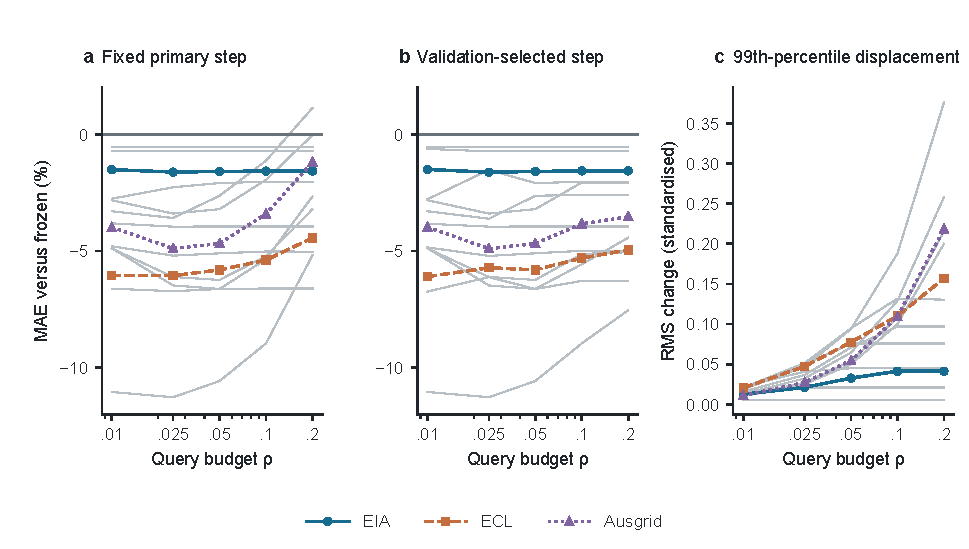
\includegraphics[width=\textwidth]{figures/fig4_budget.pdf}
\caption{\textbf{Prediction error and forecast displacement across budgets.} (a) MAE relative to frozen forecasting at the primary selected $\eta$. (b) The same comparison after validation-only selection within each $\rho$. (c) Setting-specific 99th-percentile displacement per active update at the fixed primary $\eta$. Grey curves show all 12 settings; coloured curves show dataset means with equal weights for settings. Profiles are descriptive; test outcomes do not select the budget. Disabled policies have zero correction and are recorded separately. Displacement quantiles condition on active updates. Plotting code was prepared with OpenAI Codex (CLI 0.162.0-alpha.2).}
\label{fig:budget}
\end{figure}

\FloatBarrier
\subsection{Predictive gains persist under expanded tuning}
QUART retained predictive gains across the 12 benchmark settings under expanded comparator tuning. Mean relative MAE differences were $-4.02\%$ against frozen forecasting (95\% CI, $-4.66$ to $-3.40\%$) and $-1.81\%$ against controlled COSA (95\% CI, $-2.29$ to $-1.35\%$). The difference was $-0.74\%$ against independently tuned NLMS (95\% CI, $-0.97$ to $-0.53\%$). It was $-0.13\%$ against independently tuned historical clipping (95\% CI, $-0.26$ to $-0.03\%$). Table~\ref{tab:macro} summarises MAE and RMSE; Fig.~\ref{fig:accuracy} shows the setting-level response.

\begin{table}[!htbp]
\centering\small
\caption{Benchmark mean relative differences between QUART and each comparator.}
\label{tab:macro}\begin{tabular}{lr@{\enspace}lr@{\enspace}l}
\toprule
Comparator & \multicolumn{2}{c}{Mean MAE difference (\%)} & \multicolumn{2}{c}{Mean RMSE difference (\%)}\\
\midrule
Frozen & $-4.02$ & [$-4.66, -3.40$] & $-2.21$ & [$-2.82, -1.63$]\\
Controlled COSA & $-1.81$ & [$-2.29, -1.35$] & $-1.37$ & [$-1.93, -0.90$]\\
NLMS & $-0.74$ & [$-0.97, -0.53$] & $-0.43$ & [$-0.68, -0.22$]\\
Historical clipping & $-0.13$ & [$-0.26, -0.03$] & $-0.06$ & [$-0.17, +0.04$]\\
\addlinespace[3pt]
Matched NLMS & $-5.01$ & [$-6.28, -3.65$] & $-5.41$ & [$-6.80, -3.74$]\\
Matched historical clipping & $-0.11$ & [$-0.22, -0.02$] & $-0.03$ & [$-0.12, +0.04$]\\
\bottomrule
\end{tabular}

\par\vspace{3pt}\begin{minipage}{\linewidth}\footnotesize
Negative values favour QUART. Brackets show pointwise paired 95\% seed/calendar-block intervals from seven-day blocks and 5,000 draws. Means weight the 12 settings equally; matched controls use QUART's selected step size.
\end{minipage}
\end{table}

Validation selected $\eta=1$ in 12 QUART configurations and 50 COSA update steps in 5 configurations. No COSA configuration selected starting rate 0.01. These boundary optima qualify the comparison as a finite-search result.

\begin{figure}[!htbp]
\centering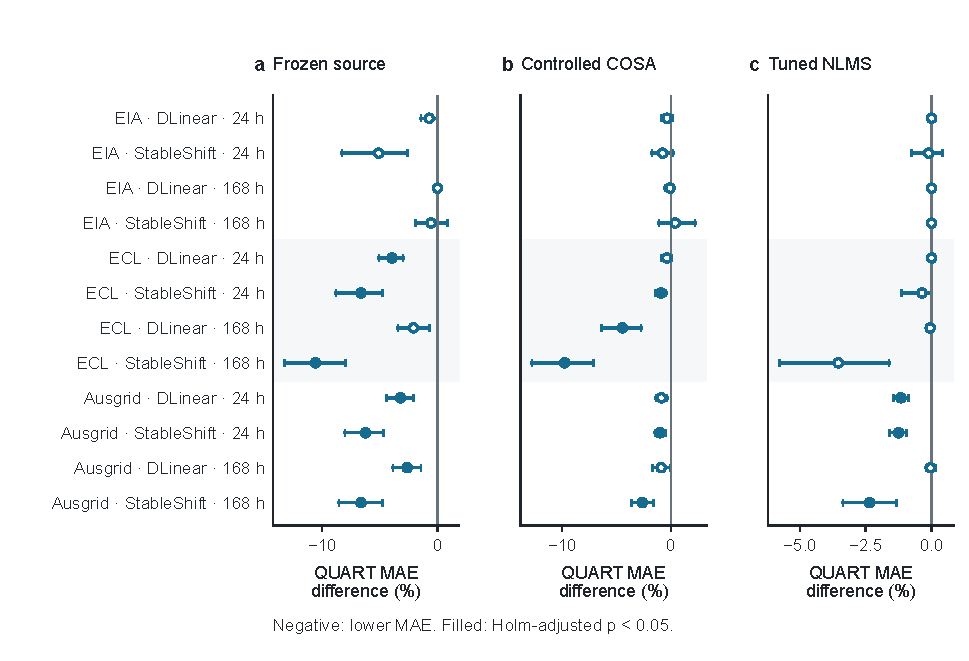
\includegraphics[width=\textwidth]{figures/fig2_expanded_accuracy.pdf}
\caption{\textbf{Prediction error across benchmark settings.} Relative QUART MAE differences from (a) frozen forecasting, (b) controlled COSA and (c) independently tuned NLMS. The display includes all 12 dataset/horizon/source settings and five source seeds. Bars show pointwise paired 95\% intervals. Filled markers meet Holm-adjusted $p<0.05$ in the 72-test MAE/RMSE family. Axis ranges differ to resolve the comparison magnitudes. Supplementary Information and Source Data report historical clipping, absolute scores and block sensitivities. Plotting code was prepared with OpenAI Codex (CLI 0.162.0-alpha.2).}
\label{fig:accuracy}
\end{figure}

\FloatBarrier
\subsection{Entity transfer reveals a cohort-dependent accuracy tradeoff}
Across eight new-entity settings, update control persisted with cohort-dependent accuracy. QUART's mean relative MAE difference was $-15.13\%$ against frozen forecasting (95\% CI, $-16.48$ to $-13.67\%$). The difference was $+2.04\%$ against fixed NLMS (95\% CI, $+0.13$ to $+4.36\%$). It was $-0.35\%$ against fixed historical clipping (95\% CI, $-0.50$ to $-0.23\%$; Fig.~\ref{fig:transfer}). Calibration configurations were fixed on the original entities before cohort preparation and scoring.

The accuracy cost was concentrated in ECL 24 h StableShift, where QUART had $+21.62\%$ higher MAE than NLMS (95\% CI, $+13.15$ to $+32.88\%$). In the primary seven-day analysis, all four Ausgrid contrasts favoured QUART and met the primary family's Holm threshold. Supplementary Section S5 reports longer-block sensitivity. Update control thus persisted across cohorts with different predictive responses. On the EIA extension, the expanded QUART/NLMS contrast was $-0.01\%$ (95\% CI, $-0.17$ to $+0.15\%$). The query constraint rarely activated in this extension (Table~\ref{tab:control_boundary}).

\begin{figure}[!htbp]
\centering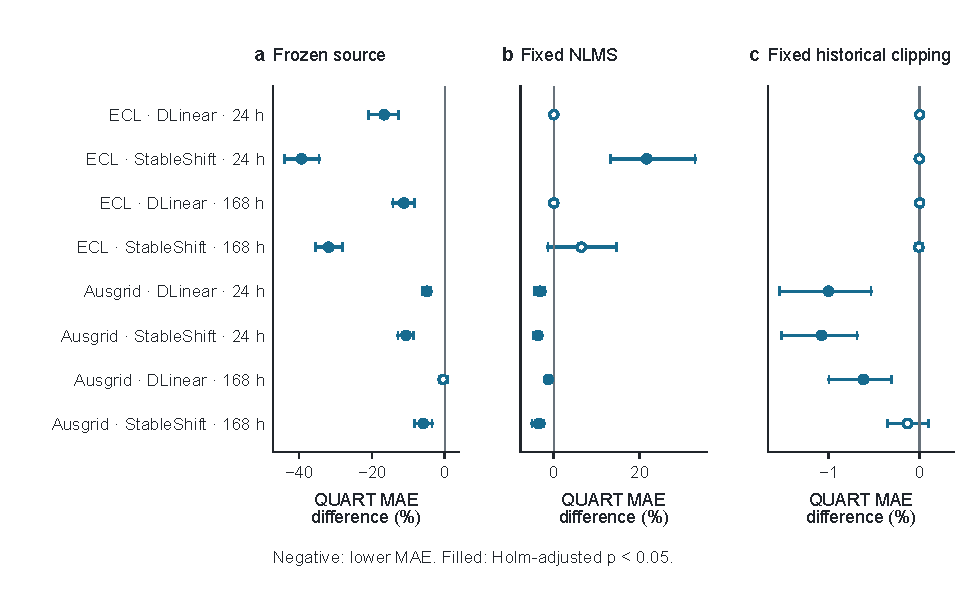
\includegraphics[width=\textwidth]{figures/fig5_entity_transfer.pdf}
\caption{\textbf{Prediction error after transfer to new entities.} Relative QUART MAE differences from (a) frozen forecasting, (b) fixed NLMS and (c) fixed historical clipping on ECL/Ausgrid entities 101--116. All eight horizon/source/cohort settings use five archived source seeds. Bars show pointwise paired 95\% seed/calendar-block intervals. Filled markers meet Holm-adjusted $p<0.05$ in the 48-test primary family for (a,b) and 16-test historical family for (c). Source models are reused without retraining, using fixed ascending-ID mapping and training-only cohort normalisation on the original calendar. Plotting code was prepared with OpenAI Codex (CLI 0.162.0-alpha.2).}
\label{fig:transfer}
\end{figure}

\FloatBarrier
\section{Discussion}
Forecast adaptation changes both prediction error and the forecast itself. QUART makes learning-induced forecast displacement an explicit control variable. Historical clipping recovered much of the predictive benefit of shrinking normalised proposals, yet allowed larger changes at the current query. Taken together, these results separate predictive accuracy from the magnitude of forecast revision.

Normalised adaptive filtering supplies the learning direction and observed-feedback descent \parencite{nagumo1967}. QUART brings prediction-space step control \parencite{schulman2015trpo} to frozen output calibration with delayed supervision \parencite{kim2025tta,im2026cosa,wang2026fac}. An affine effective operator removes redundant gated parameterisation and exposes the permitted step in closed form. Matured feedback sets the learning direction, while the current query sets the step limit. The resulting interface links forecast-change budgets to online learning without source-model backpropagation.

Training scaling coefficients translate the budget into physical units. If $s_{\max}$ is the largest channel standardisation scale, one update has joint physical-unit RMS displacement at most $s_{\max}B_t$. A physical tolerance $\tau$ therefore gives the sufficient standardised budget $B_t\leq\tau/s_{\max}$. The original Ausgrid cohort has a median analytical envelope of 0.0601 kWh per hourly interval under the recorded primary budget. Supplementary Section S5 gives the conversion for every cohort. Entity transfer retained the bound even when accuracy relative to NLMS worsened, illustrating why both properties require evaluation.

The bound applies to one update at a fixed query in joint-channel, training-standardised coordinates. Expanded temporal comparisons remain exploratory, and entity transfer uses the same historical calendar with a fixed positional mapping. New temporal cohorts and irregular feedback with actual publication delays would test whether the accuracy--displacement response extends to other operating conditions. Supplementary Information gives the full evaluation design and provenance.

\Needspace{9\baselineskip}
\section{Conclusion}
QUART turns each delayed-feedback learning step into a bounded revision of the current forecast. Its closed-form rule preserves observed-feedback descent, and matched controls show that similar prediction error can accompany different update magnitudes. Entity transfer maintains the bound while revealing a cohort-dependent accuracy tradeoff. Forecast revision can thus be specified alongside accuracy when designing and evaluating online adaptation.

\section*{Data availability}
EIA-930, ECL and Ausgrid are publicly available from the cited providers. Generated Source Data, including error sums and counts, paired statistics and forecast-change measurements, is deposited in version 0.4.0 of the research archive \parencite{qorc2026materials}. The release is available at \url{https://github.com/bianyanbo44-afk/stable-shift-forecasting/releases/tag/quart-v0.4.0}. Source Data also accompanies the manuscript.
\section*{Code availability}
Source forecasters, 60 selected checkpoints, and calibration and evaluation code are available in the same versioned archive \parencite{qorc2026materials}. A reproduction package, including the current figure scripts, accompanies the manuscript.
\section*{CRediT authorship contribution statement}
Yanbo Bian: Conceptualization, Methodology, Software, Validation, Formal analysis, Investigation, Data curation, Visualization, Writing -- original draft, Writing -- review \& editing. Zhihai Wang: Supervision, Writing -- review \& editing.
\section*{Funding}
This research received no specific grant from funding agencies in the public, commercial, or not-for-profit sectors.
\section*{Declaration of competing interest}
The authors declare that they have no known competing financial interests or personal relationships that could have appeared to influence the work reported in this paper.
\section*{Supplementary material}
Supplementary Information provides proofs, data and source-model specifications, complete comparisons, sensitivity analyses and reproduction instructions.
\section*{Declaration of generative AI and AI-assisted technologies in the manuscript preparation process}
During the preparation of this work, the authors used OpenAI Codex for software development, literature searches, statistical workflows, figure preparation and manuscript drafting. The authors reviewed and approved the AI-assisted content and take full responsibility for the manuscript.
\renewcommand{\bibfont}{\fontsize{10}{12}\selectfont}
\setlength{\bibitemsep}{2pt}
\clearpage
\printbibliography

\end{document}
